\documentclass[../TinyBot.tex]{subfiles}
\begin{document}

\section{Construction} \label{sec:construction}

The first step is to cut out your base material. This can be any material stiff enough to support the Arduino, breadboard, and motors. The club provides corflute, though other materials such as wood or plastic from milk bottles can be used if desired. The base can be any shape, though ensure it is big enough to fit the breadboard, the Arduino you are using if not using a Nano, and a battery.
It is useful to lay out the components you are using on the base material before cutting. \\

Once you have cut out the base, peel the backing paper from the breadboard and stick the breadboard to the base.
\begin{center}
    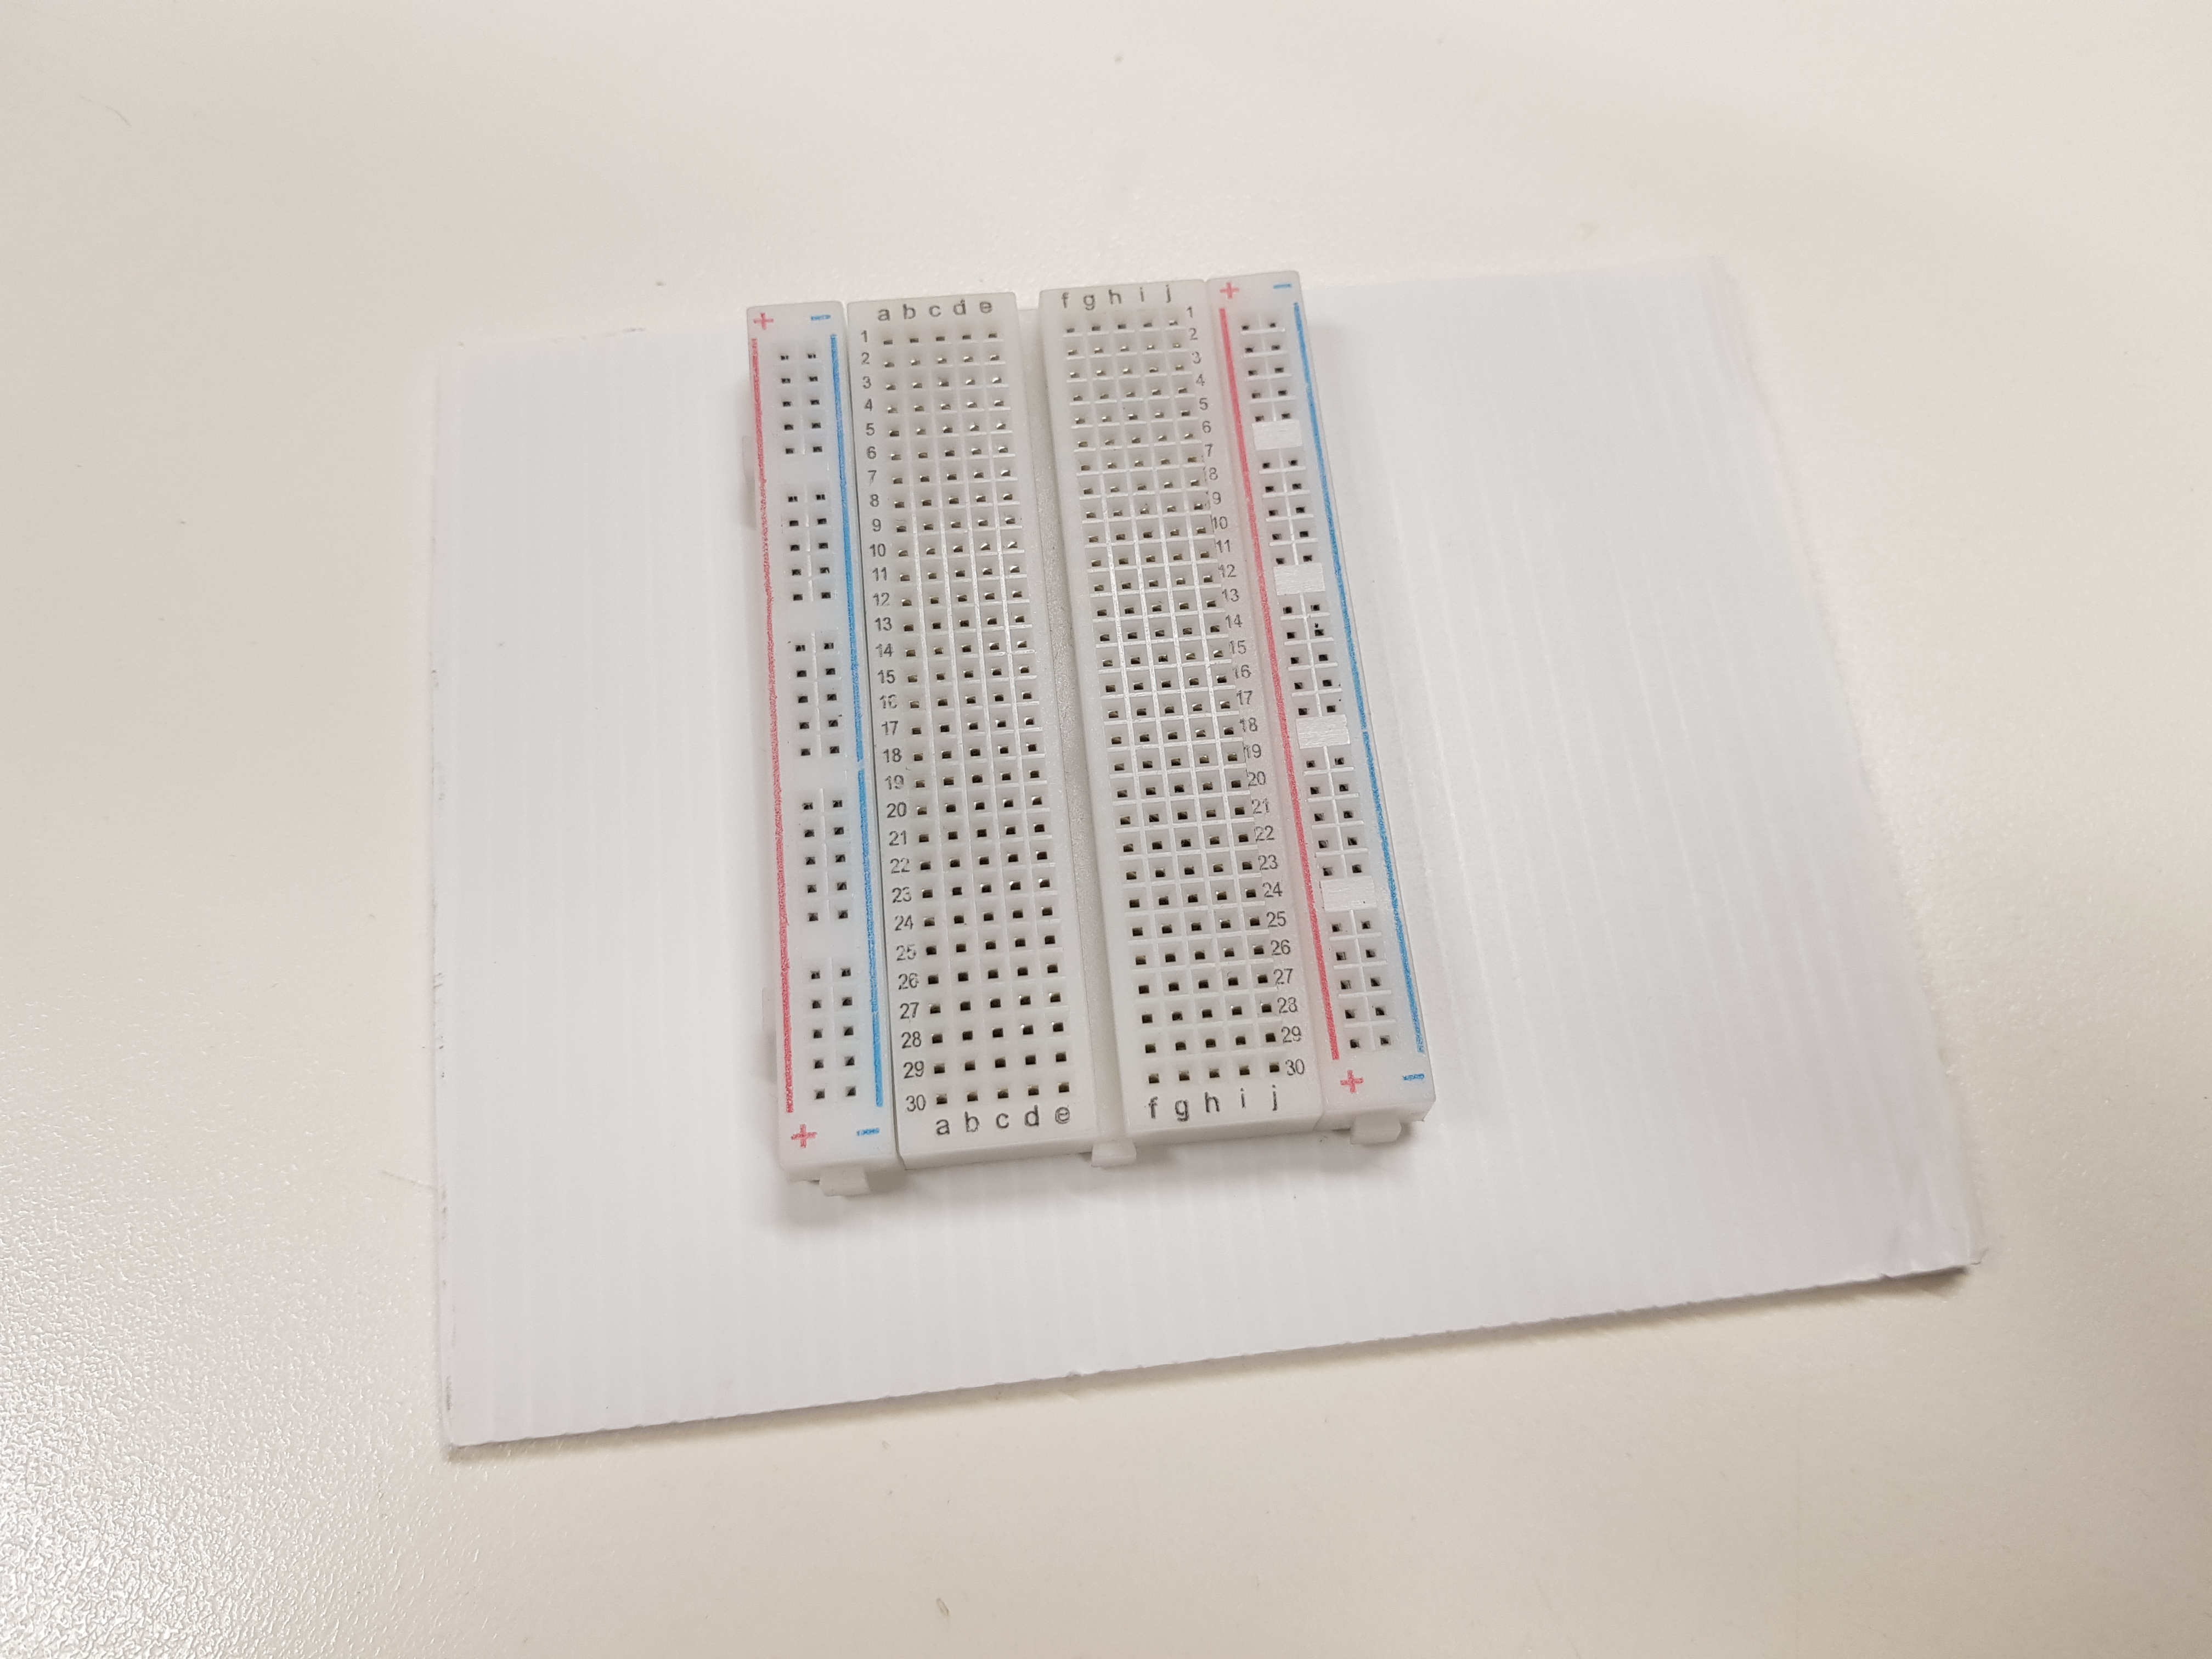
\includegraphics[width=0.6\linewidth]{breadboard_on_base.jpg}
    % \captionof{figure}{fig:construction:breadboard-on-base}
    % \label{fig:construction:breadboard-on-base}
\end{center}

Then place the motor covers and caster wheel on the base and mark out where holes need to be made. The club has plenty of motor covers, though cable ties can be used as an alternative to secure the motors. \\
If using a material like corflute the holes can be marked/made with a screwdriver. Holes will have to be marked and made differently if using other materials. 
\begin{center}
    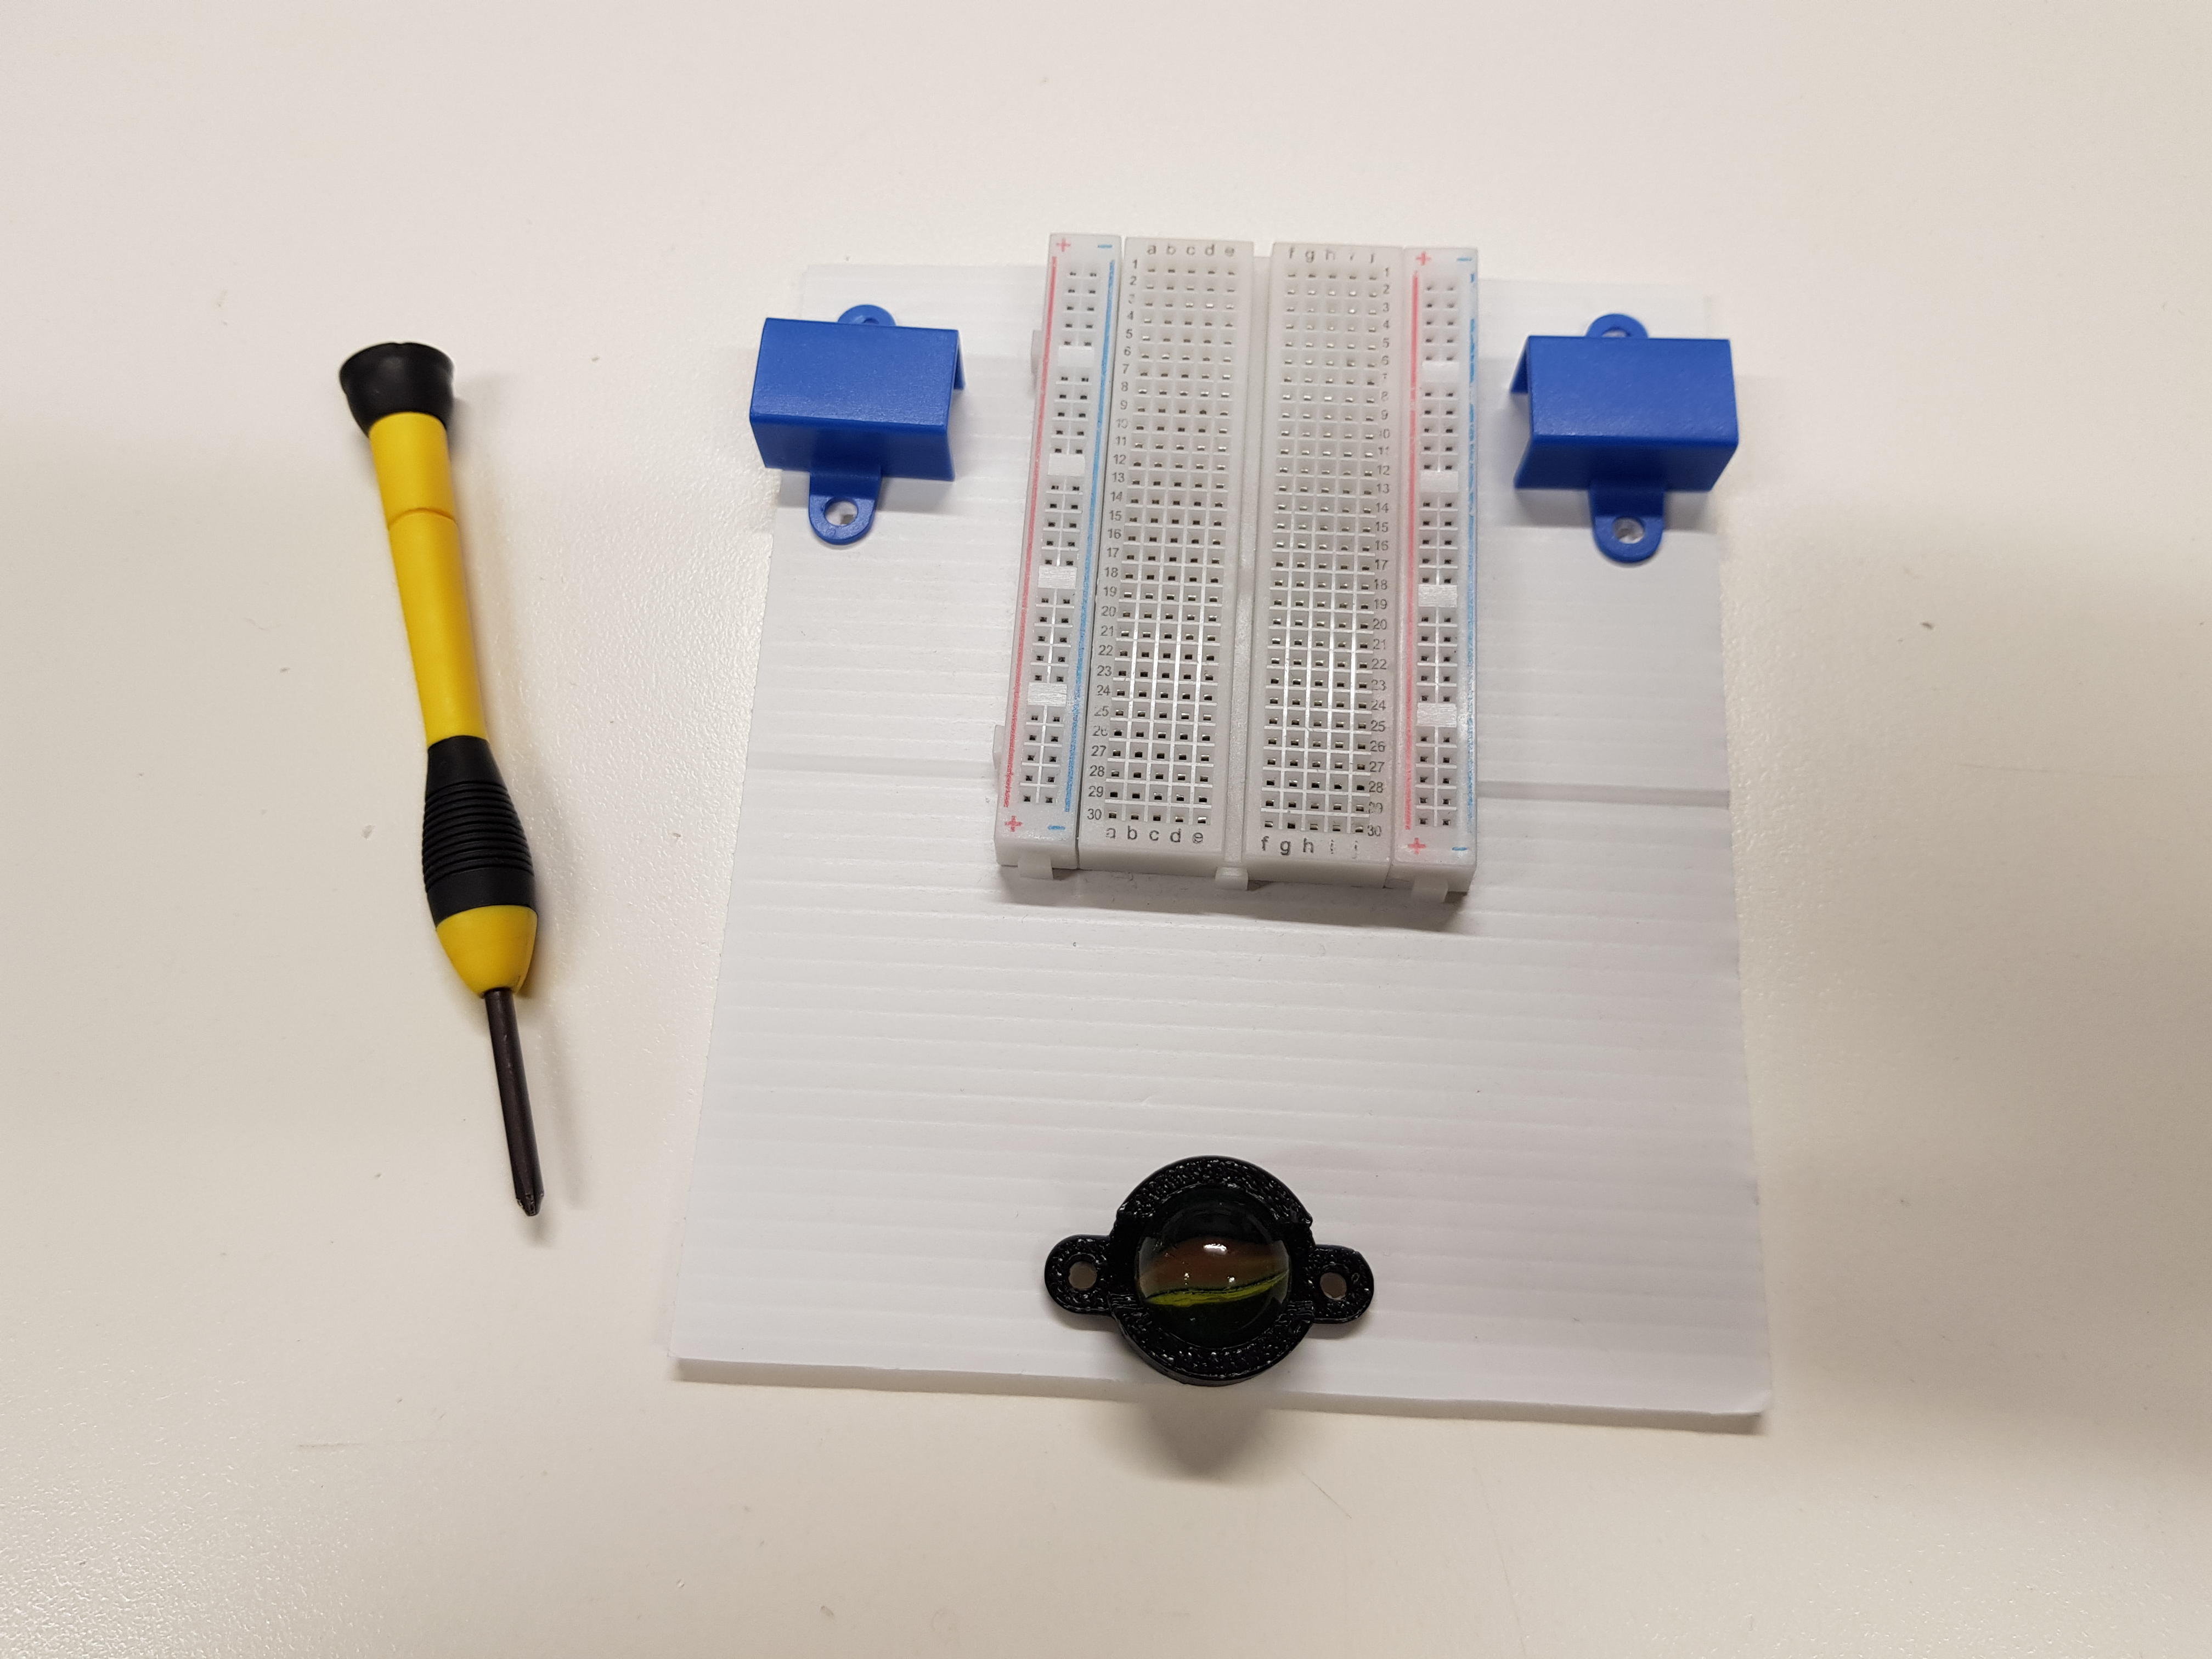
\includegraphics[width=0.6\linewidth]{lining_up_holes_base_screwdriver.jpg}
\end{center}
\begin{center}
    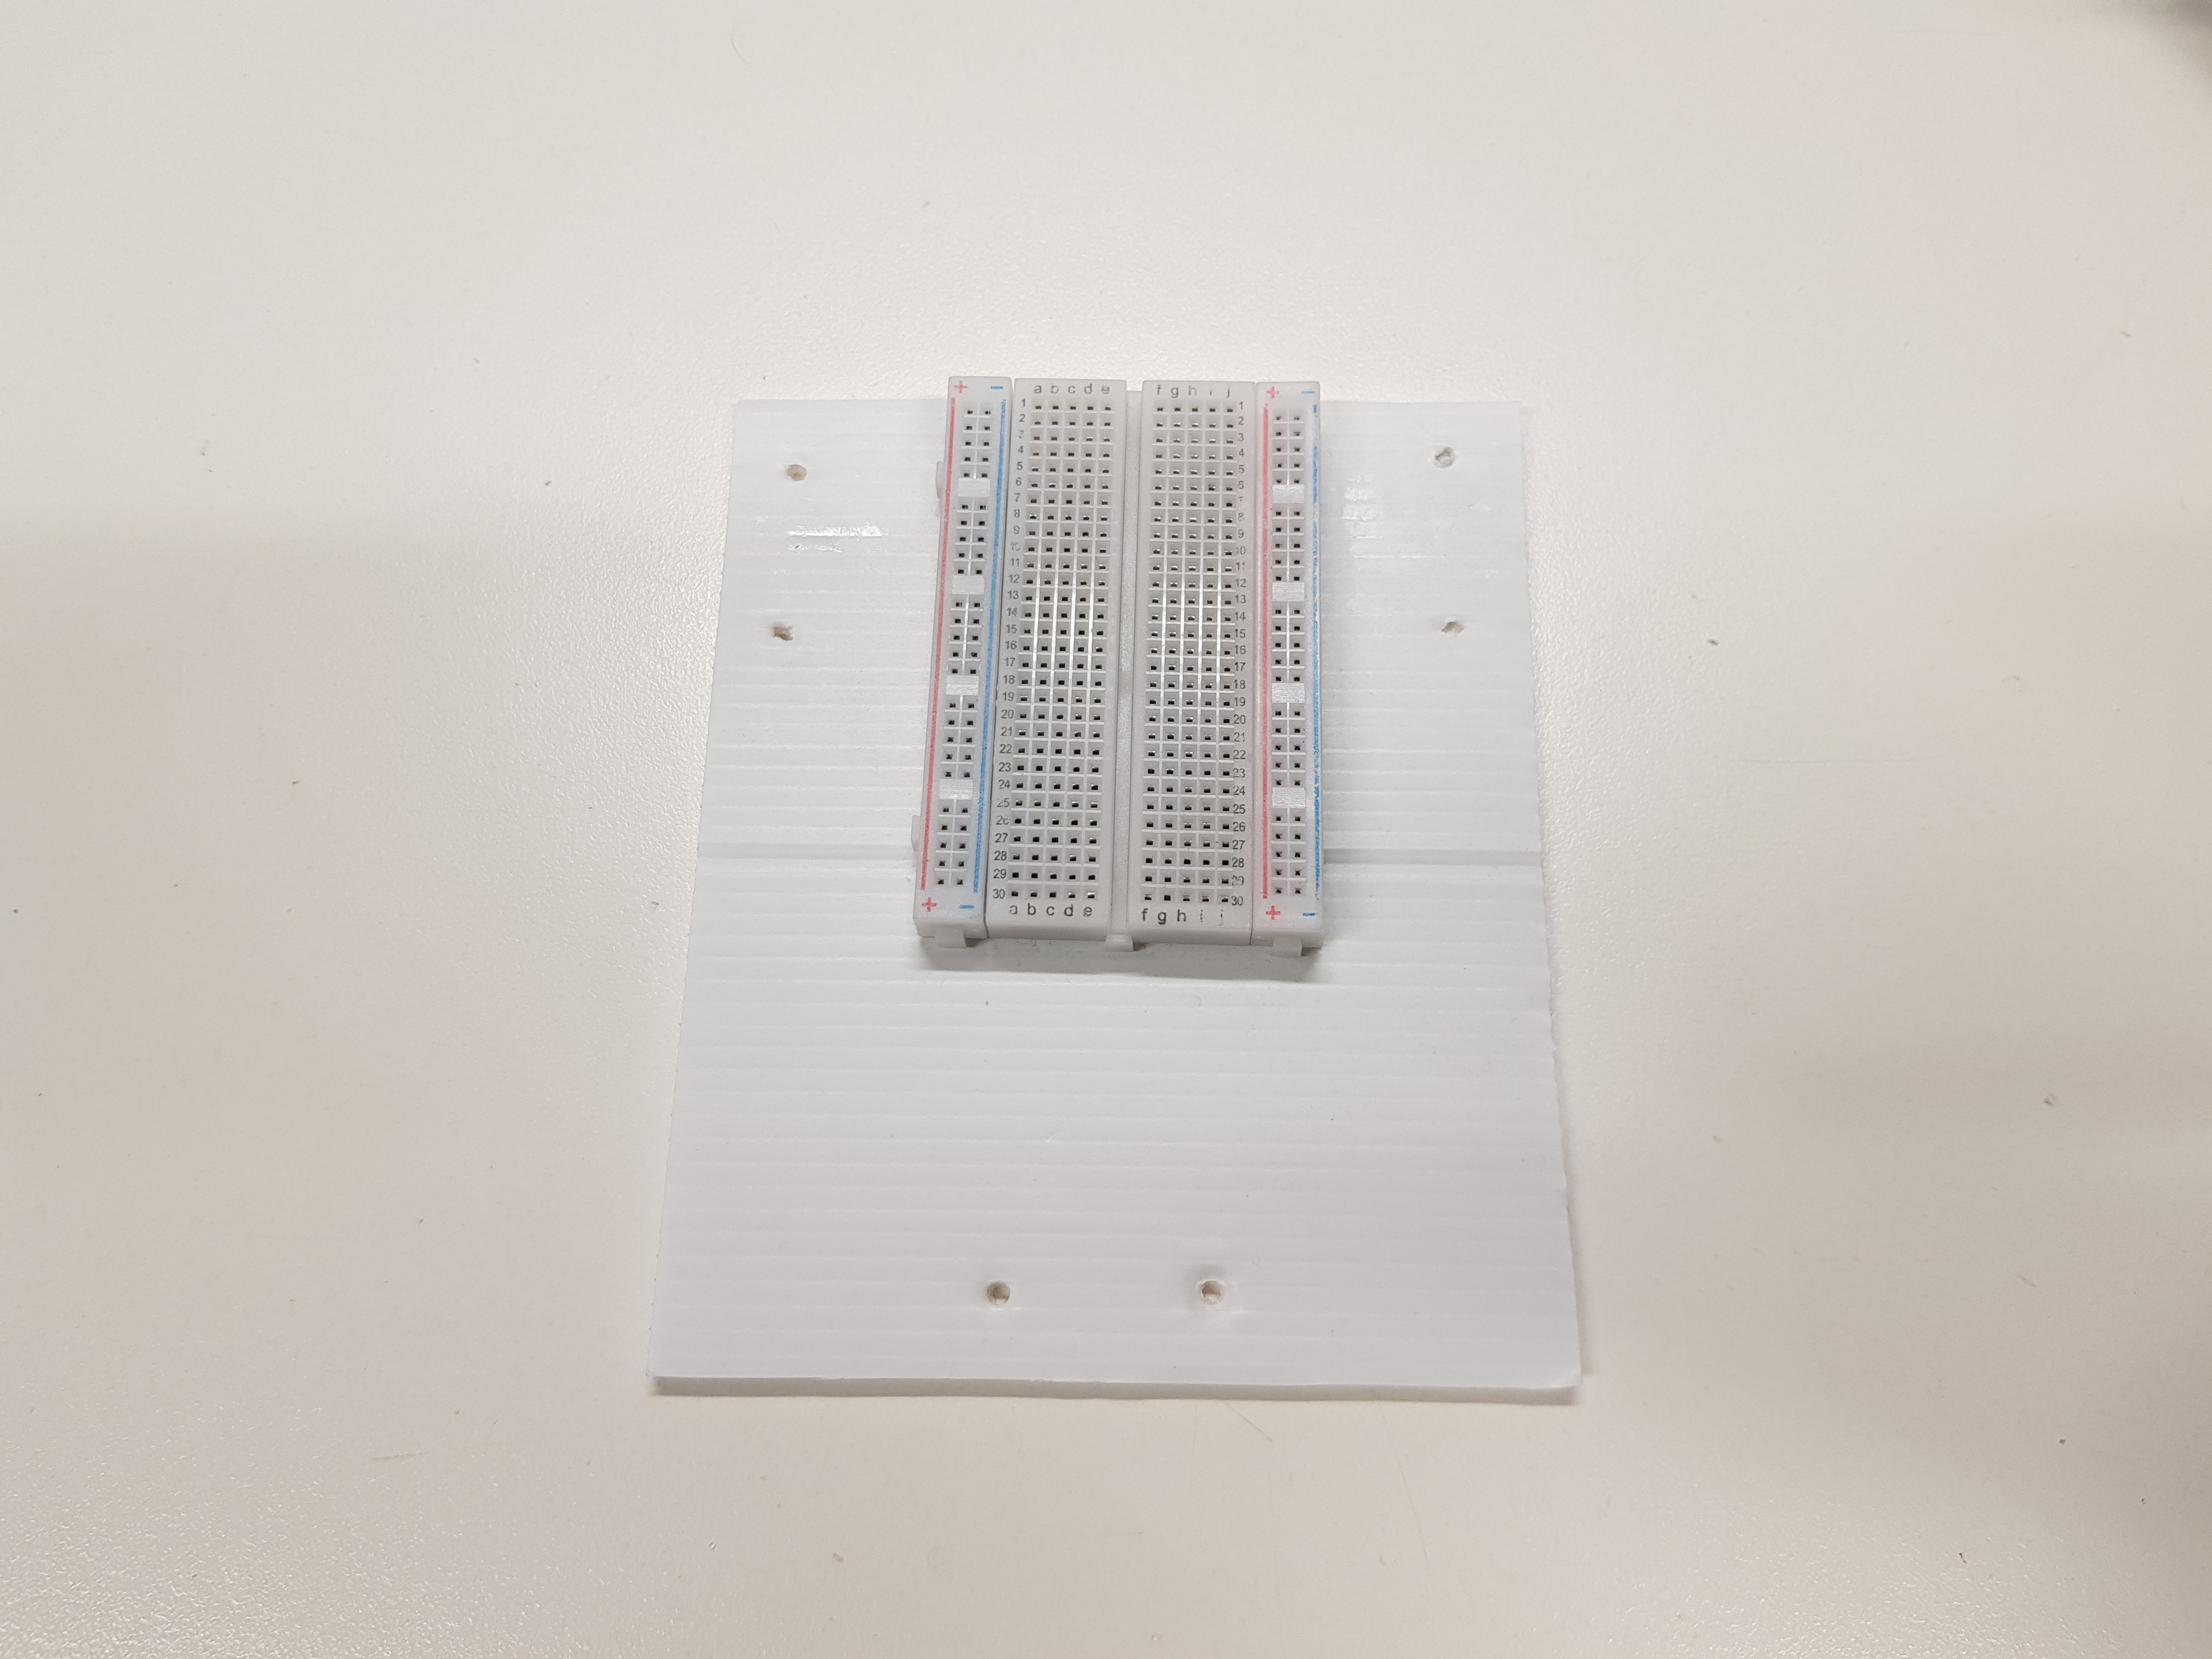
\includegraphics[width=0.6\linewidth]{base_with_holes.jpg}
\end{center}

It is much easier to assemble the circuit on a flat base when the robot has the wheels and caster wheel attached. 

% At this point it is easiest to assemble the circuit on the breadboard. 

\begin{center}
    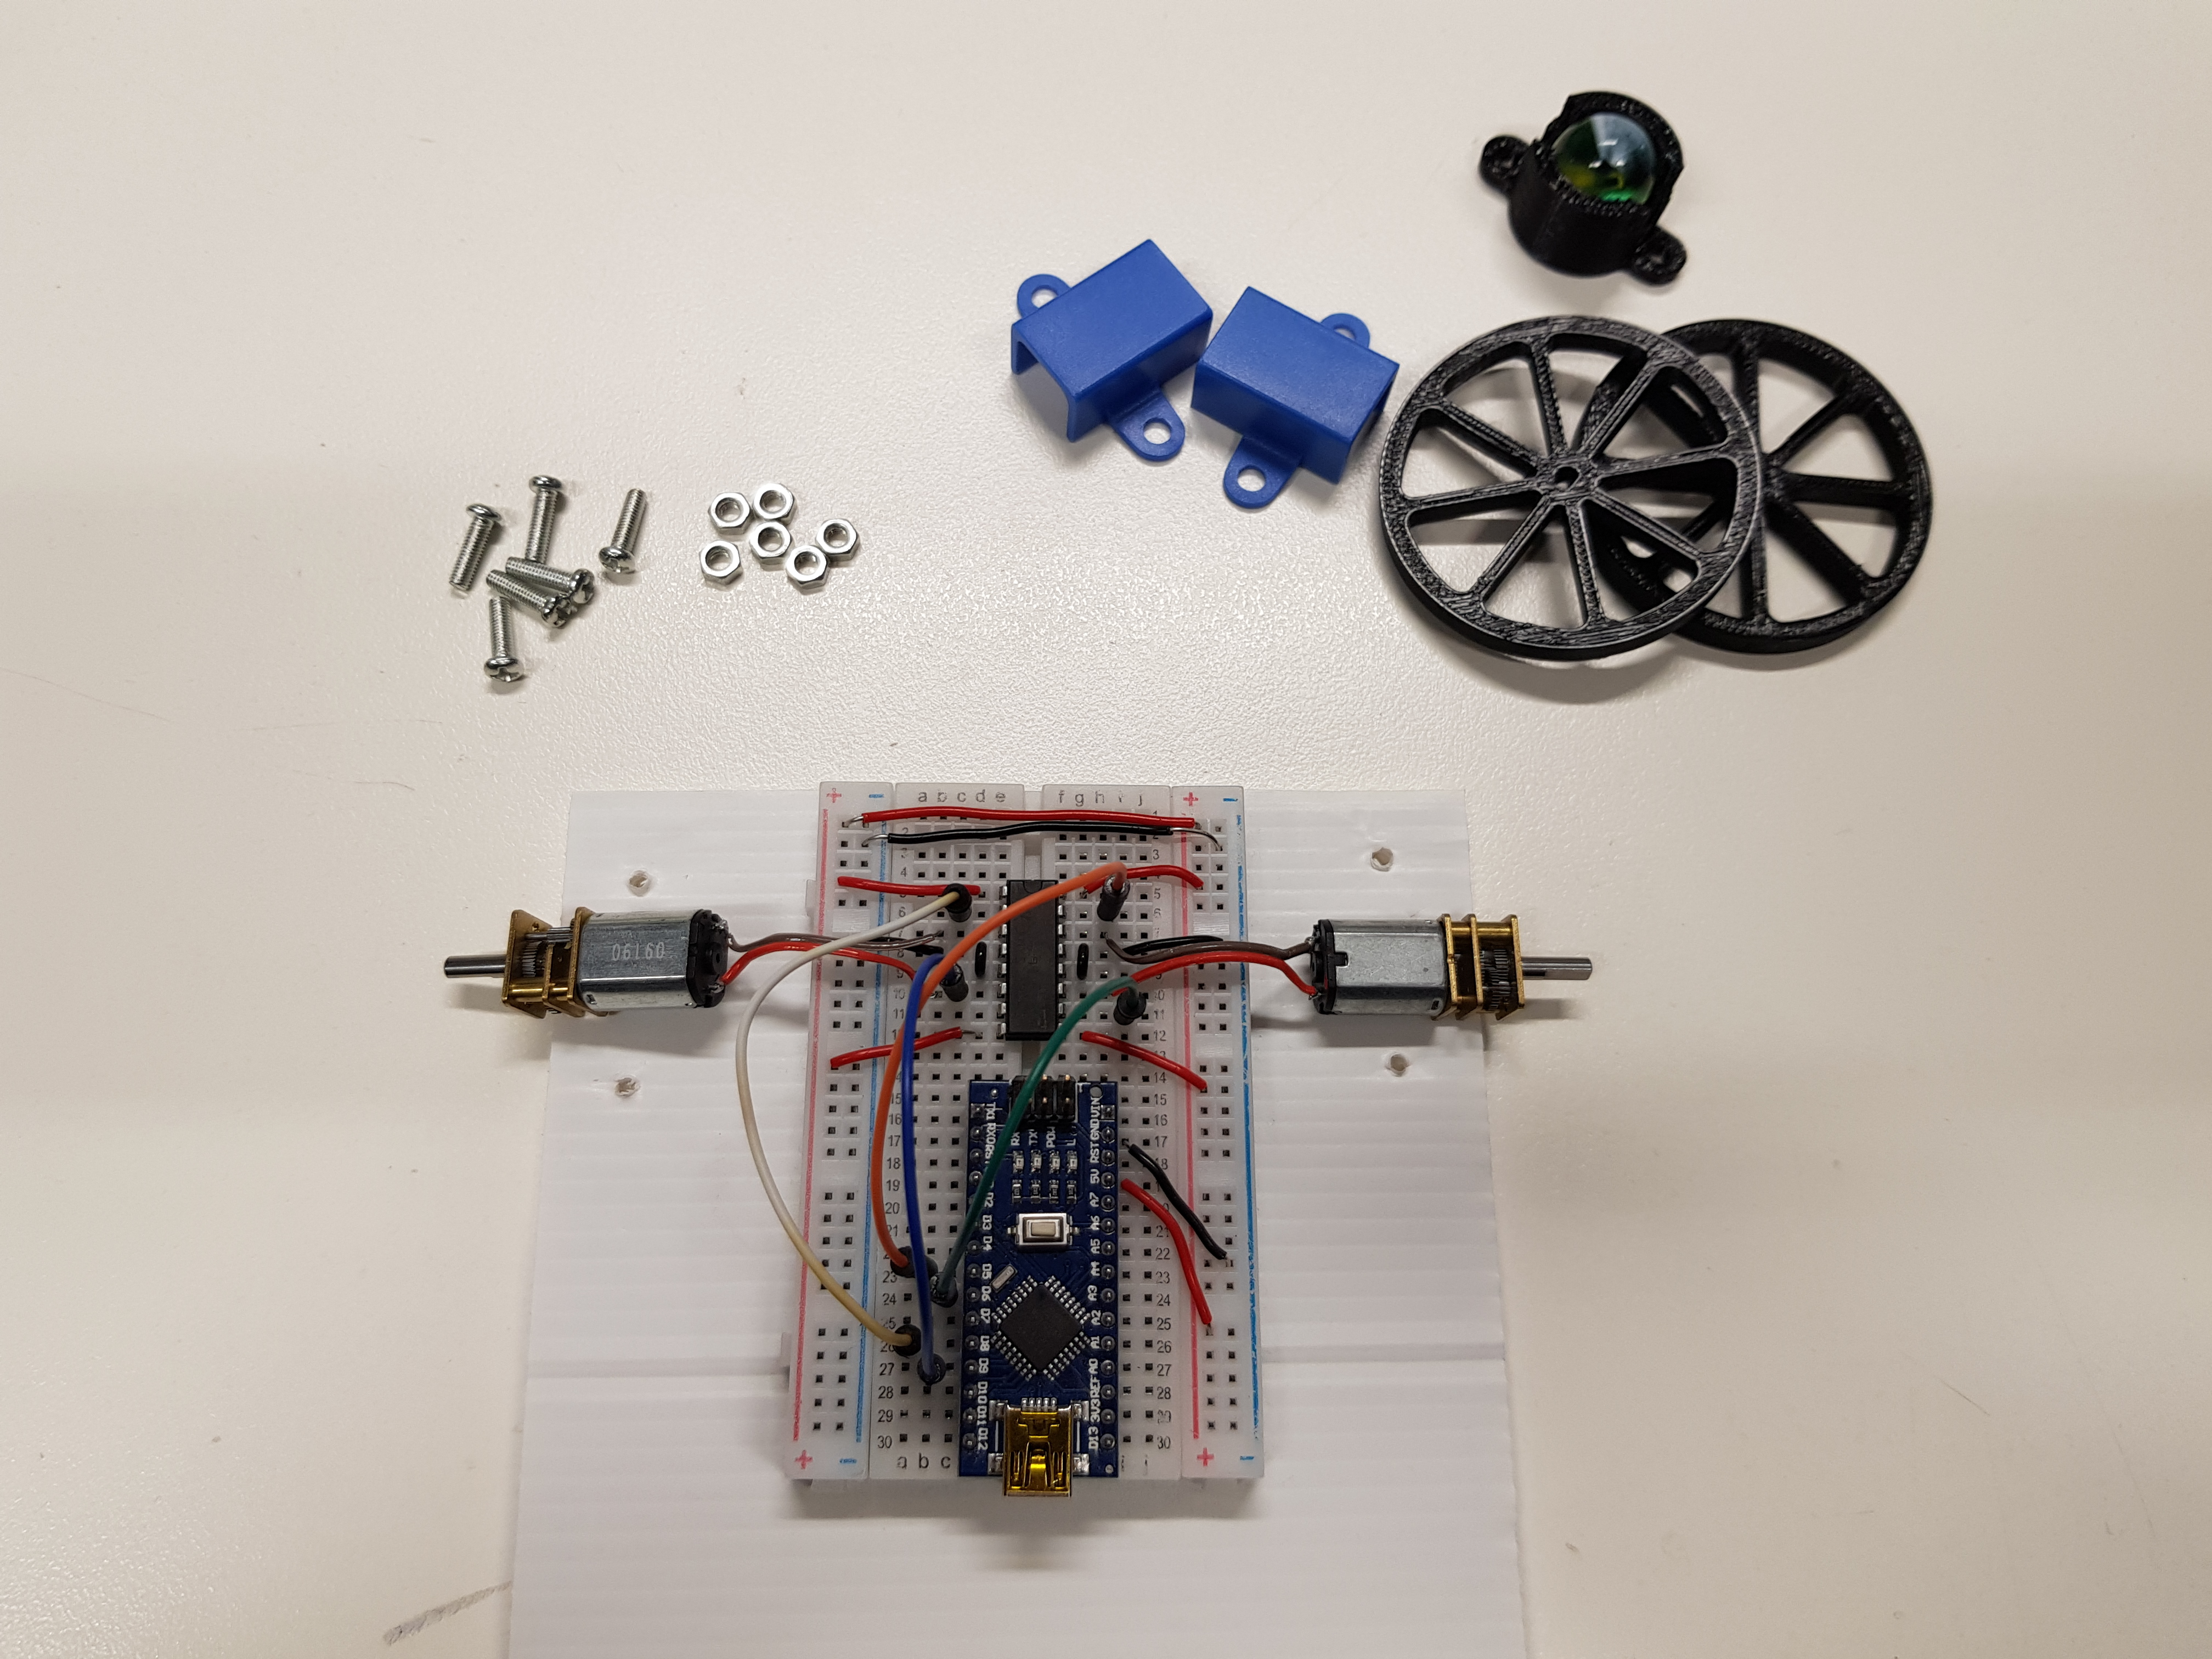
\includegraphics[width=0.6\linewidth]{wired_all_parts.jpg}
\end{center}
Place the motor covers over the motors and attach to the base using the provided screws. The caster wheel is also attached using screws. 
% \begin{center}
%     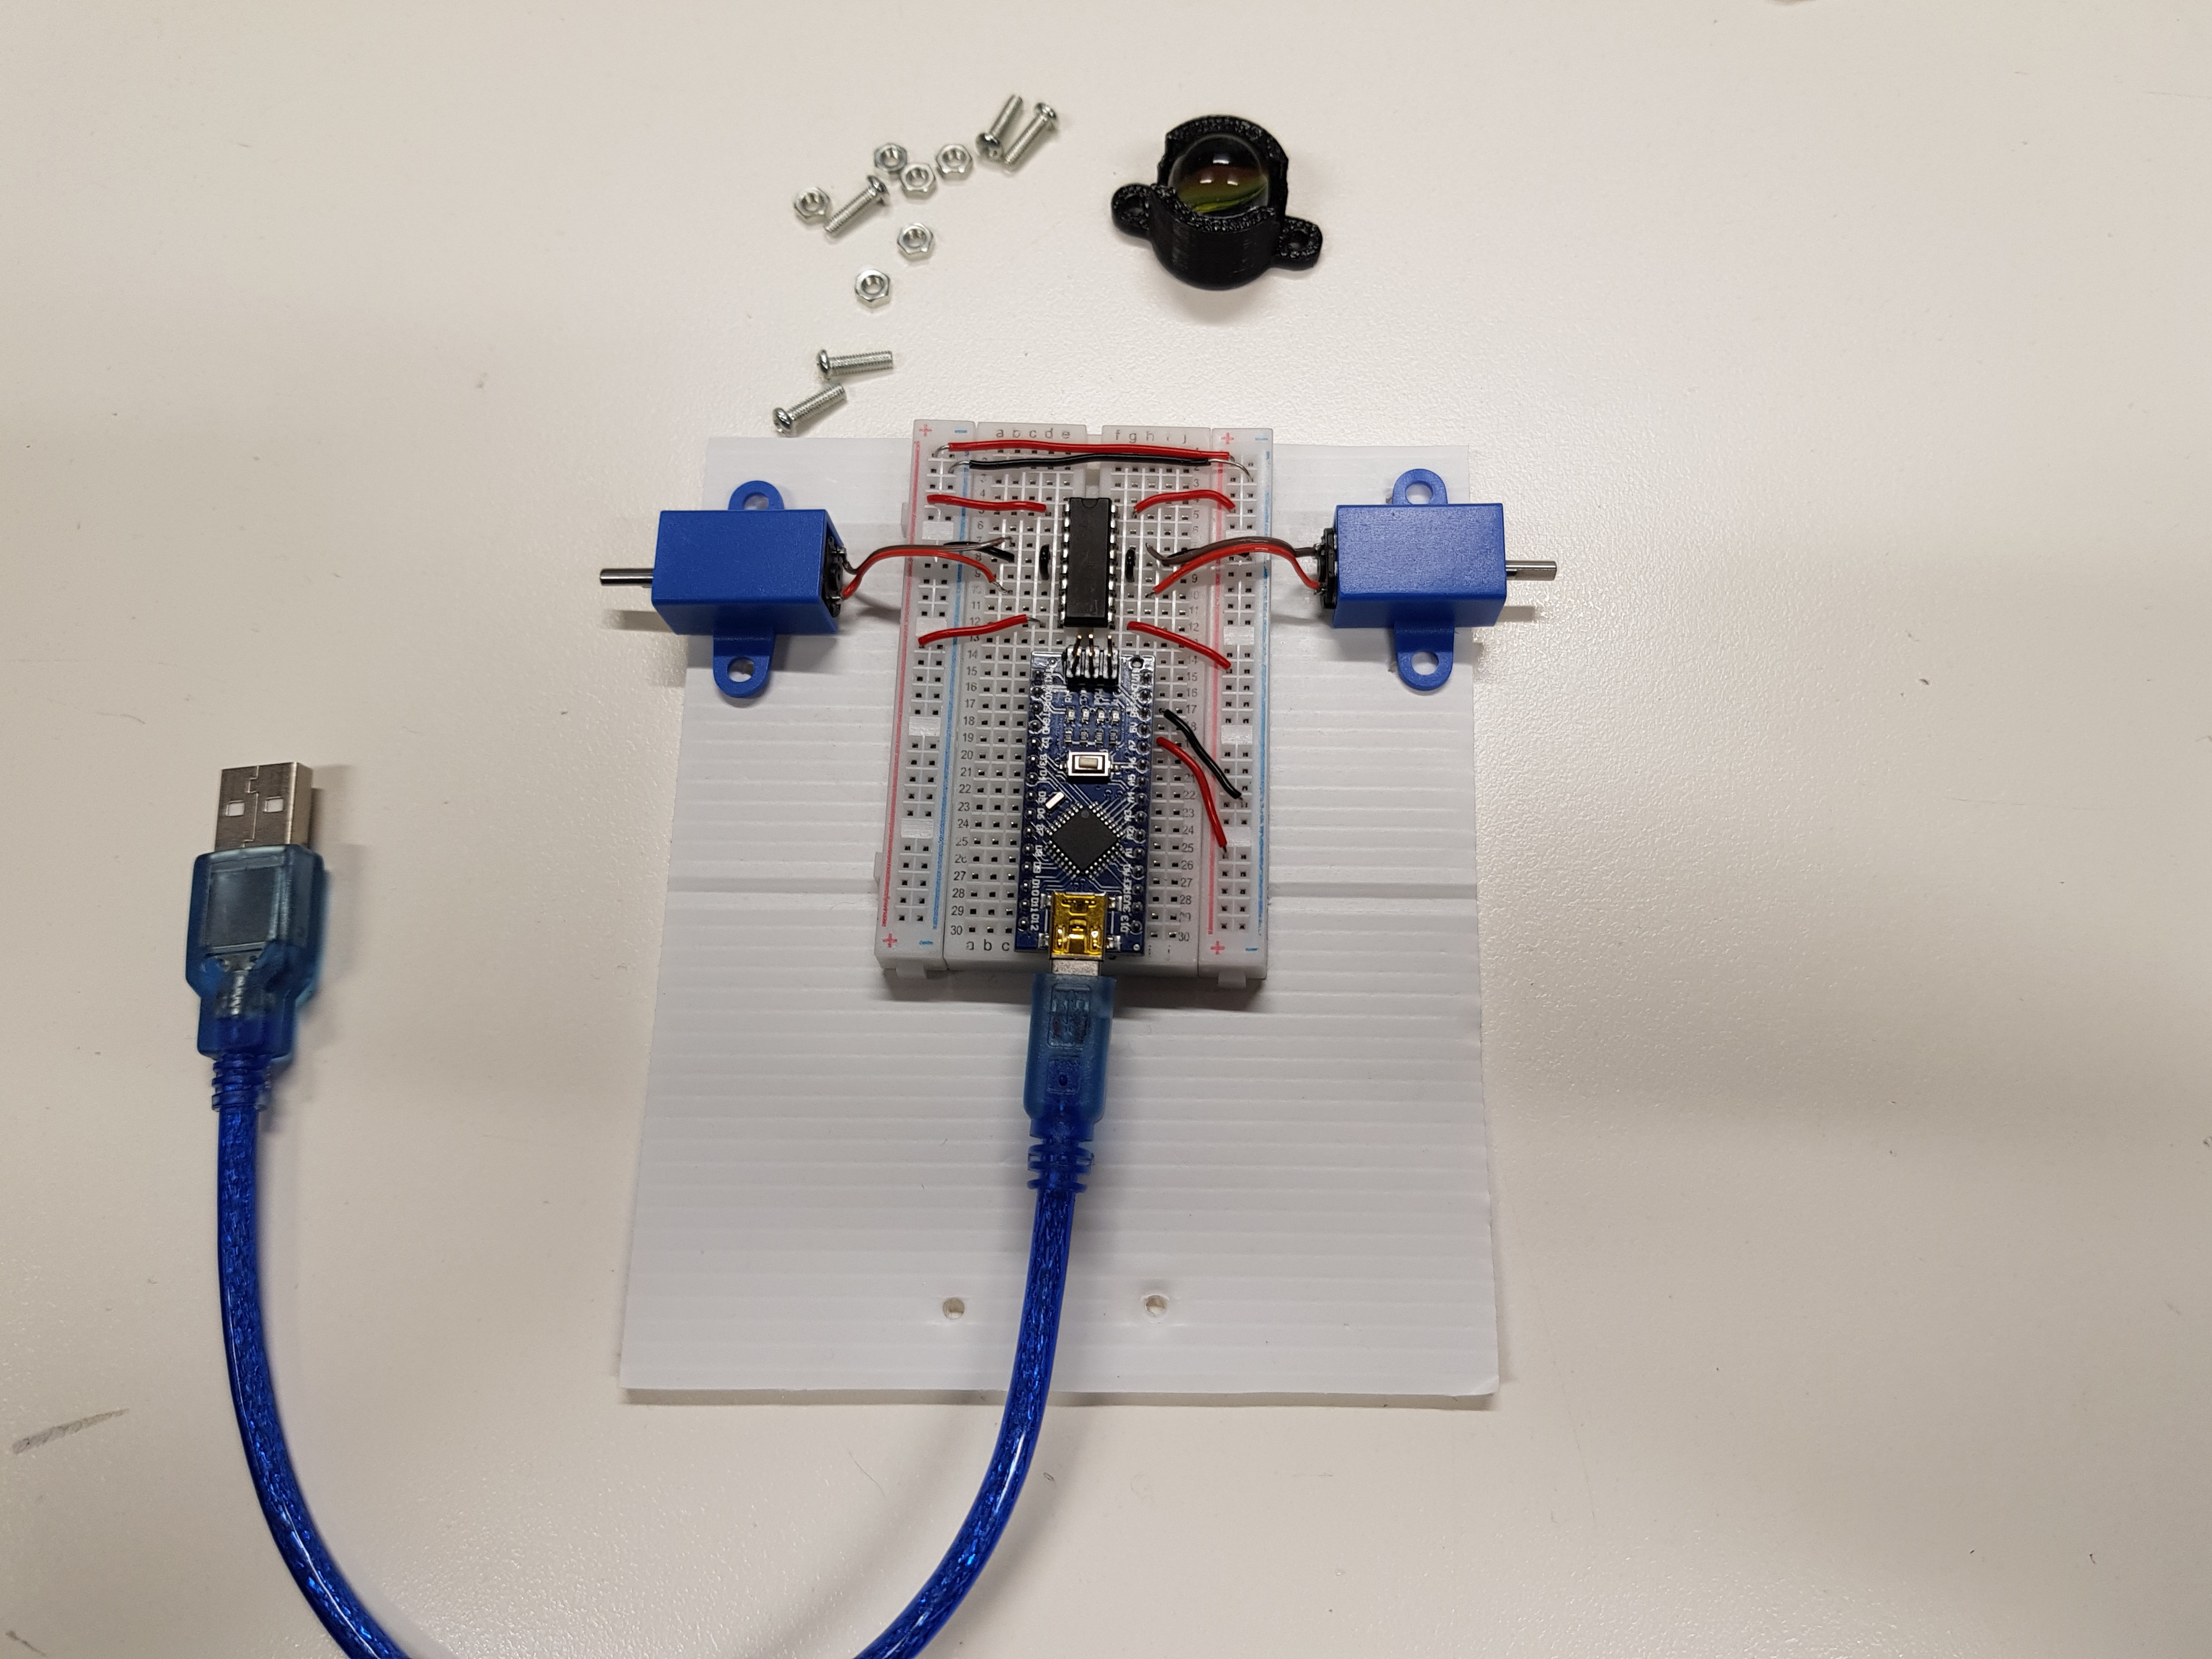
\includegraphics[width=0.6\linewidth]{circuit_base_all_parts_minus_wheels.jpg}
% \end{center}

\begin{center}
    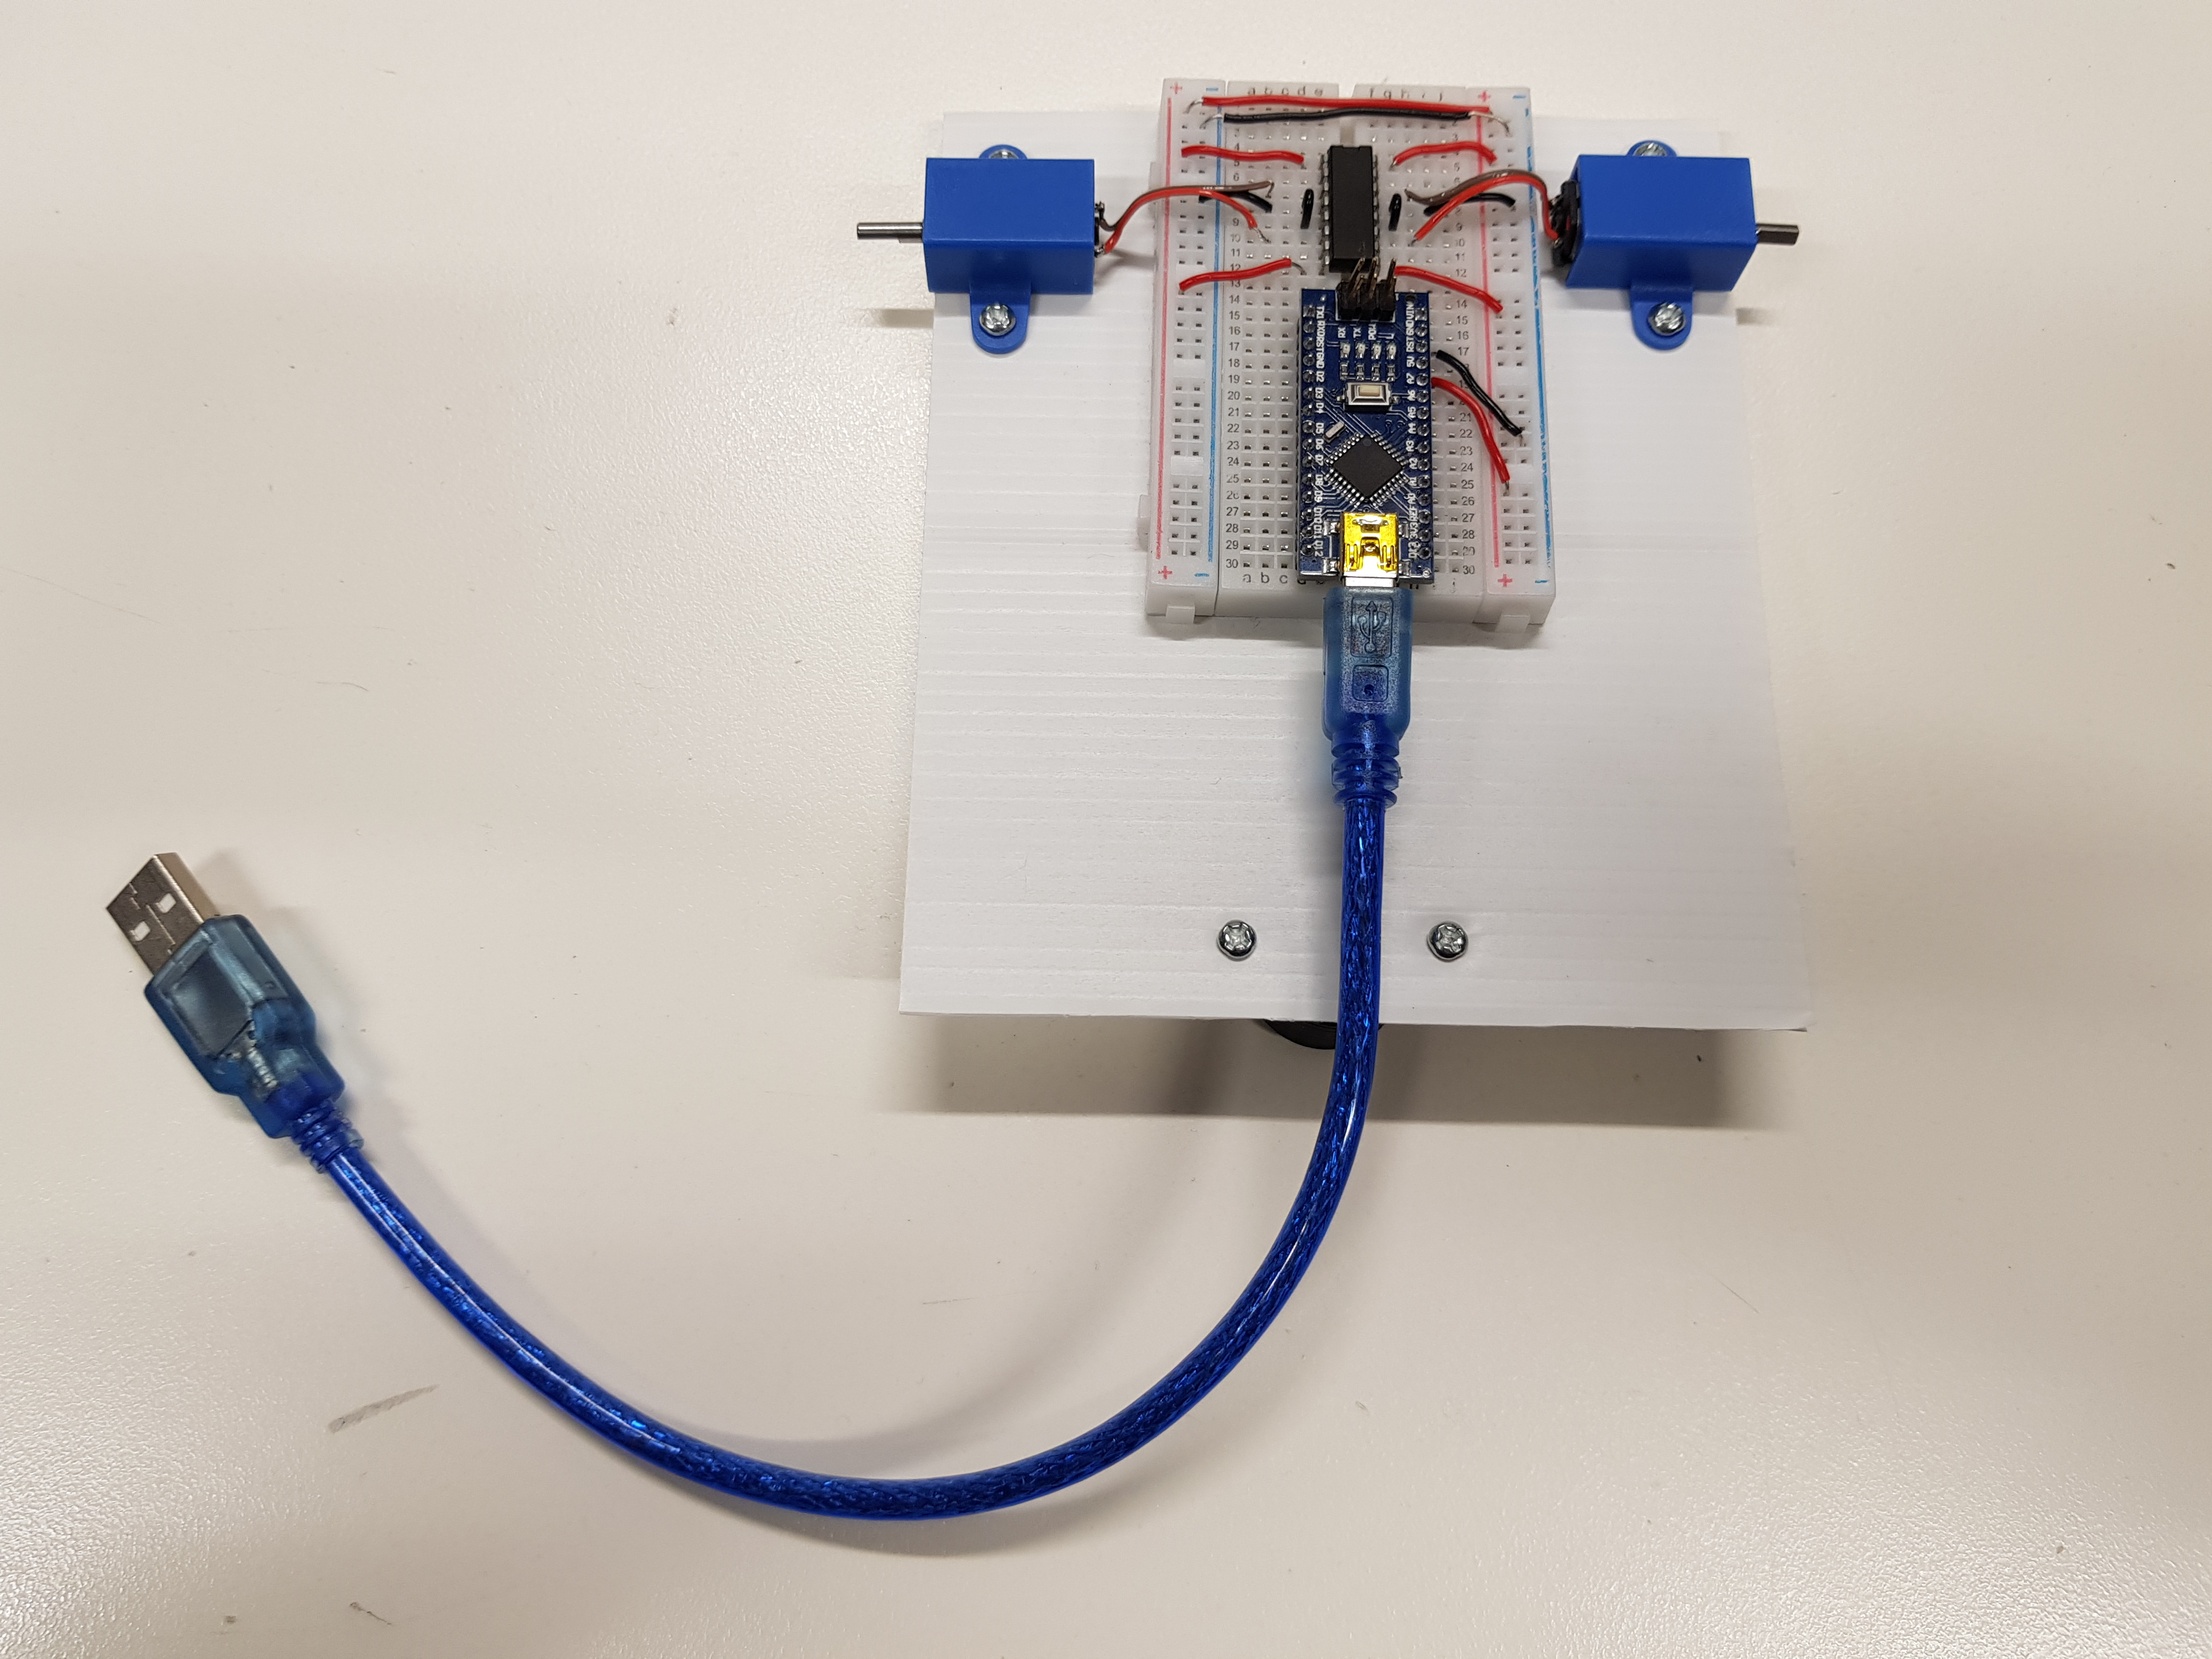
\includegraphics[width=0.6\linewidth]{cover_and_caster_screws.jpg}
\end{center}

Your TinyBot is now fully assembled.
\begin{center}
    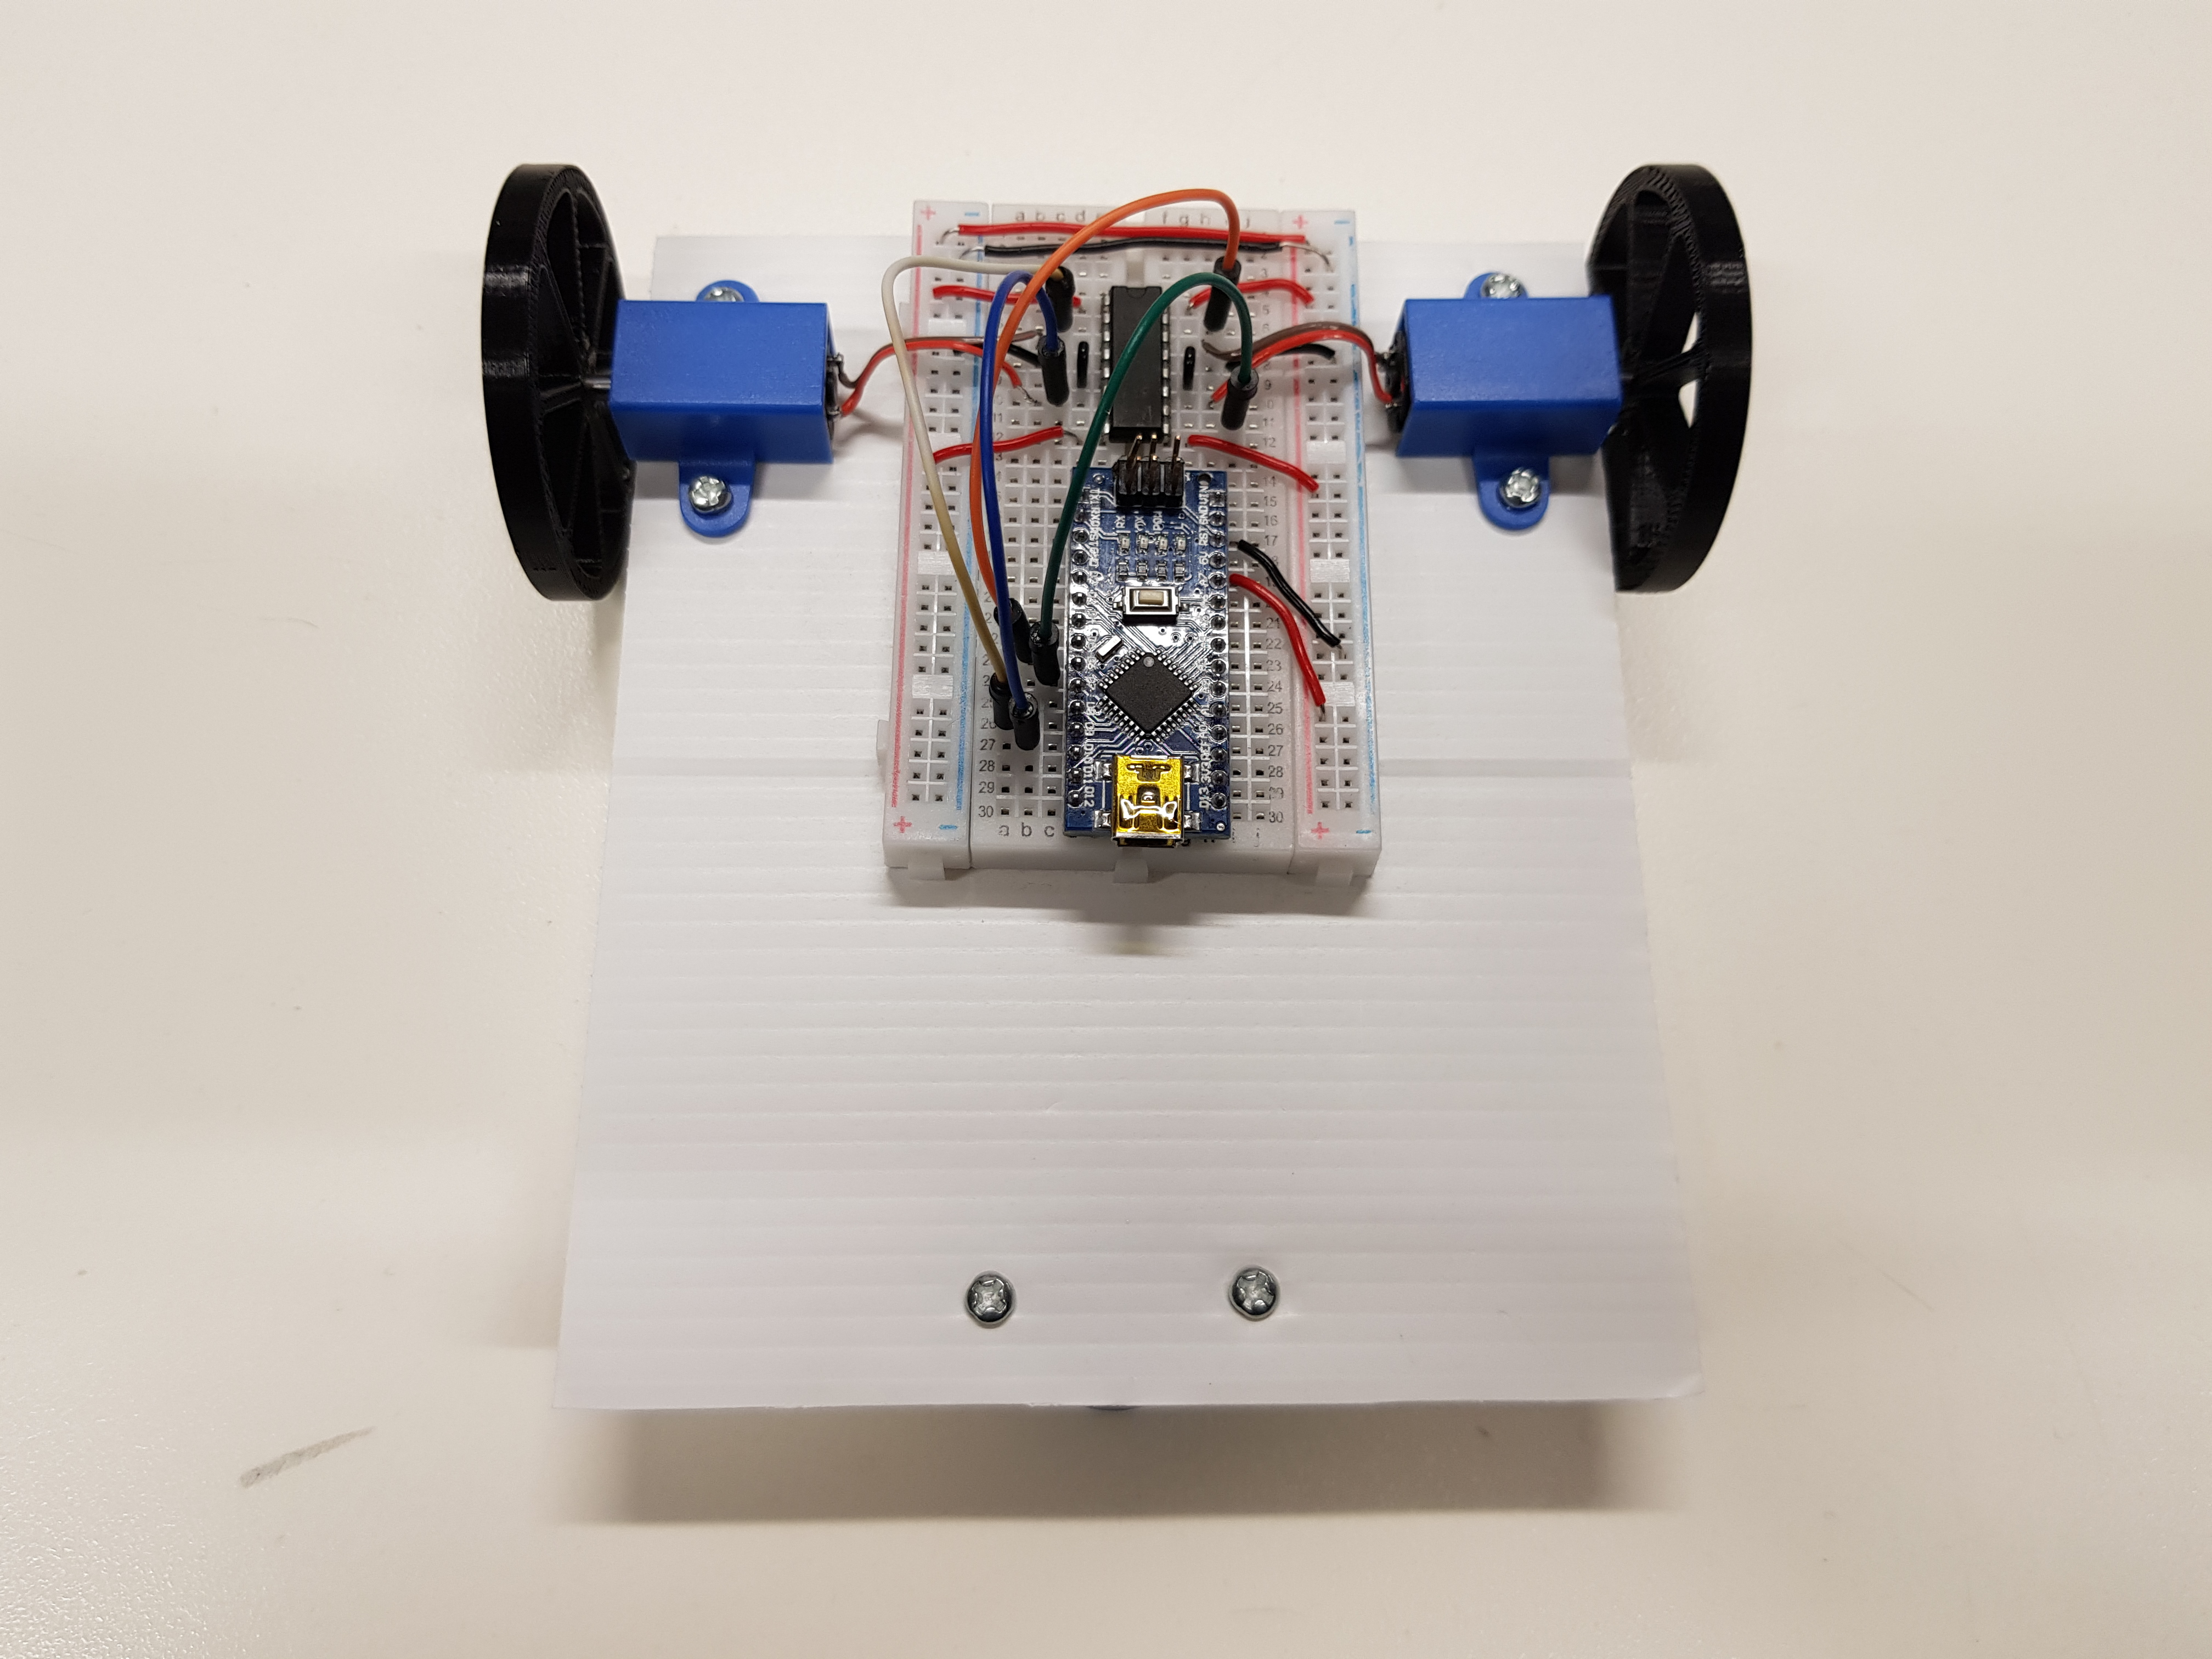
\includegraphics[width=0.6\linewidth]{final_assembled.jpg}
\end{center}

\end{document}